% !TEX encoding = UTF-8
% !TEX TS-program = pdflatex
% !TEX root = ../Tesi.tex
% !TEX spellcheck = it-IT

%************************************************
\chapter{Acustica di san Luca: ricostruzione e perdita}
\label{cap:acustica}
%************************************************

%\begin{flushright}{\slshape
%  una citazione} \\ \medskip
%    --- un tizio
%\end{flushright}

~
\vfill

Nel processo di scelta ed elaborazione del materiale sonoro volto alla costruzione del brano,
mi è subito apparso ovvio intraprendere il cammino partendo non tanto dalle qualità timbriche
del sassofono o dall'astratta struttura e forma del brano, quanto dalle qualità intrinseche
del luogo come La chiesa di San Luca e Martina.

L'analisi di questo sistema acustico è incentrato nella sua ricostruzione tridimensionale,
virtualizzazione delle sue componenti, successivamente stratificate alla sala da concerto,
assieme alla registrazione dell'environment: anche per quest'ultimo sarà posto l'accento
sulla possibile riproduzione tridimensionale.

\begin{figure}[h]
\centering
{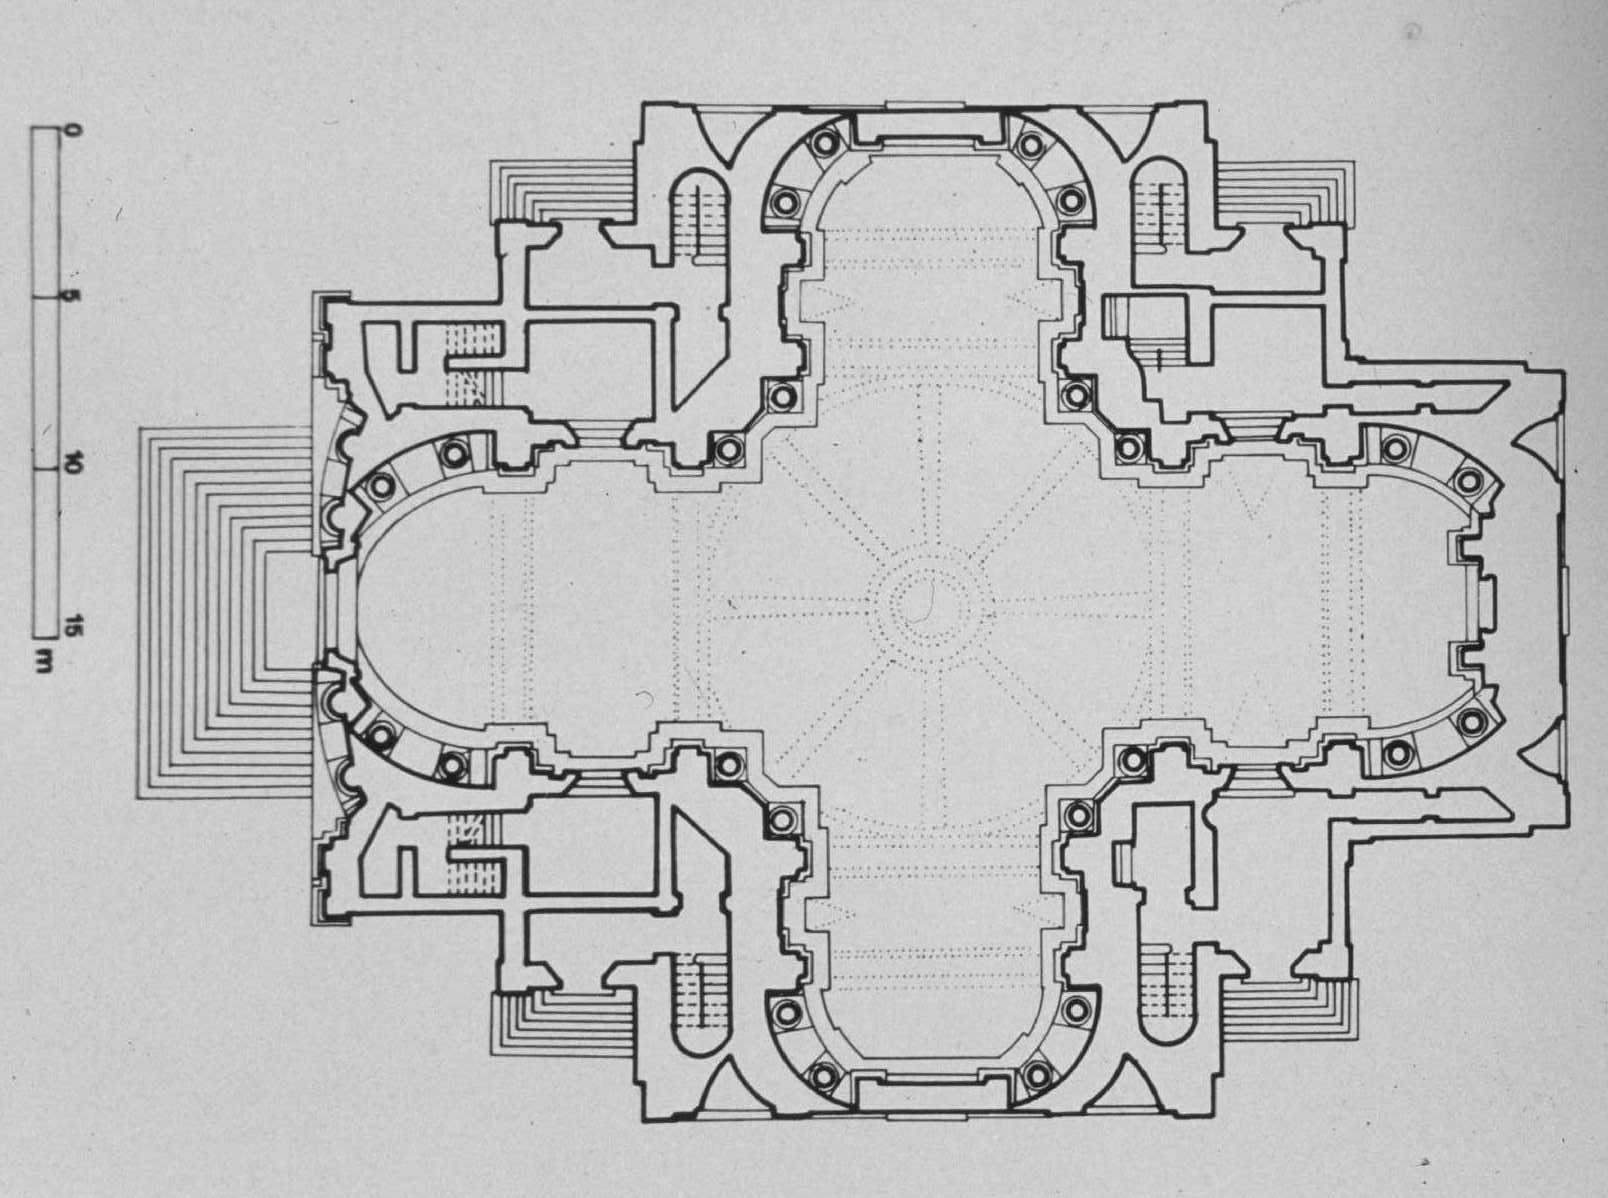
\includegraphics[width=.99\columnwidth]{04-Luca-Martina-pianta.jpg}}
\caption[Pianta S. Luca]{Pianta S. Luca}
\label{fig:tetratetra}
\end{figure}

\clearpage

\section{Cenno storico - scientifico}
\label{sec:storico}

Progettata nel 1635 da Pietro Berrettini da Cortona, la chiesa è composta da un unitaria
pianta cruciforme, che poggia sul titolo primitivo di Santa Martina, fondata nel VII
secolo da papa Onorio I, frontale all'arco di Settimio Severo. 

I due luoghi comunicano tramite il lucernario di Santa Martina e la scelta  di portare sopra
di esso l'altoparlante per l'indagine acustica, riguarda anche la ripresa delle riflessioni 
che avvengono nella chiesa inferiore e modificano l'ambiente sovrastante.
Per quanto riguarda i materiali è stato fatto affidamento alle fonti trovate all'accademia
di San Luca, nell'ipotesi di un nuovo sopralluogo e determinare, in base alle percentuali
di materiale nelle varie sezioni della chiesa il relativo livello di assorbimento della
chiesa e i conseguenti tempi delle prime  riflessioni

Materiali preponderanti della chiesa:

\begin{itemize}
	\item mattoni cotto
	\item marmo
\end{itemize}

I fenomeni principali acustici che vengono posti all'analisi riguardano:

\begin{enumerate}
	\item[a)] \textbf{il campo libero}, ovvero la distanza tra lo strumento/sorgente e gli ascoltatori. 
Stiamo parlando del confronto con il suono diretto e recepito dall'ascoltatore. Possiamo calcolarlo come:

\begin{equation}
I_{direct} = \frac{QW_{source}}{4\pi r^2}
\end{equation}

	\begin{description}
		\item[$I$] = intensità del suono diretto calcolato in watts per $m2$
		\item[$Q$] = direzionalità della sorgente 
		\item[$W$] = potenza della sorgente calcolata in watt 
		\item[$r$] = Distanza in $m^2$
	\end{description}
		
	\item[b)] \textbf{il campo riverberante}, ovvero l'energia successiva a quella diretta; prime riflessioni e coda.

\end{enumerate}

Ricordiamo che le prime riflessioni differiscono dal suono diretto sia per tempo (circa $80ms$) che direzione:


\begin{quoting}
The amount of energy, or power, removed by a given area of absorbing material will depend on the energy,
or power, per unit area striking it. As the sound intensity is a measure of the power per unit area this
means that the intensity of the sound reflected is reduced in proportion to the absorption
coefficient%\footcite{howjamie:acu}
\end{quoting}

importante è anche sottolineare come i materiali descritti in precedenza siano analizzati e ricondotti ad
una misurazione della riflessione “regionale”, specifica ai punti del quadrato, raccogliendo informazioni
riguardo alle differenti future risposte registrate.

Le mappe, descritte successivamente, riconducono a scelte di preparazione date dalla conformazione della
prima sala ove sarà eseguito il brano per la prima volta. Il sassofonista si trovava ad una
distanza di circa la metà dei metri cui sono stati disposti i microfoni per catturare le  riflessioni dello spazio.	

Il riverbero e le riflessioni della stanza sono il nostro argomento principale, ma l'analisi vedrà solo
l'attuazione di determinati punti sonori in regime e non tutta la pianta.
Schroeder a questo proposito spiega come %[DA SCRIVERE MEGLIO misura del ltempo di riverbero p. 15 /farina]
è possibile ricavare il tempo di decadimento (T60) tramite integrale della risposta all'impulso.

\begin{figure}
\centering
{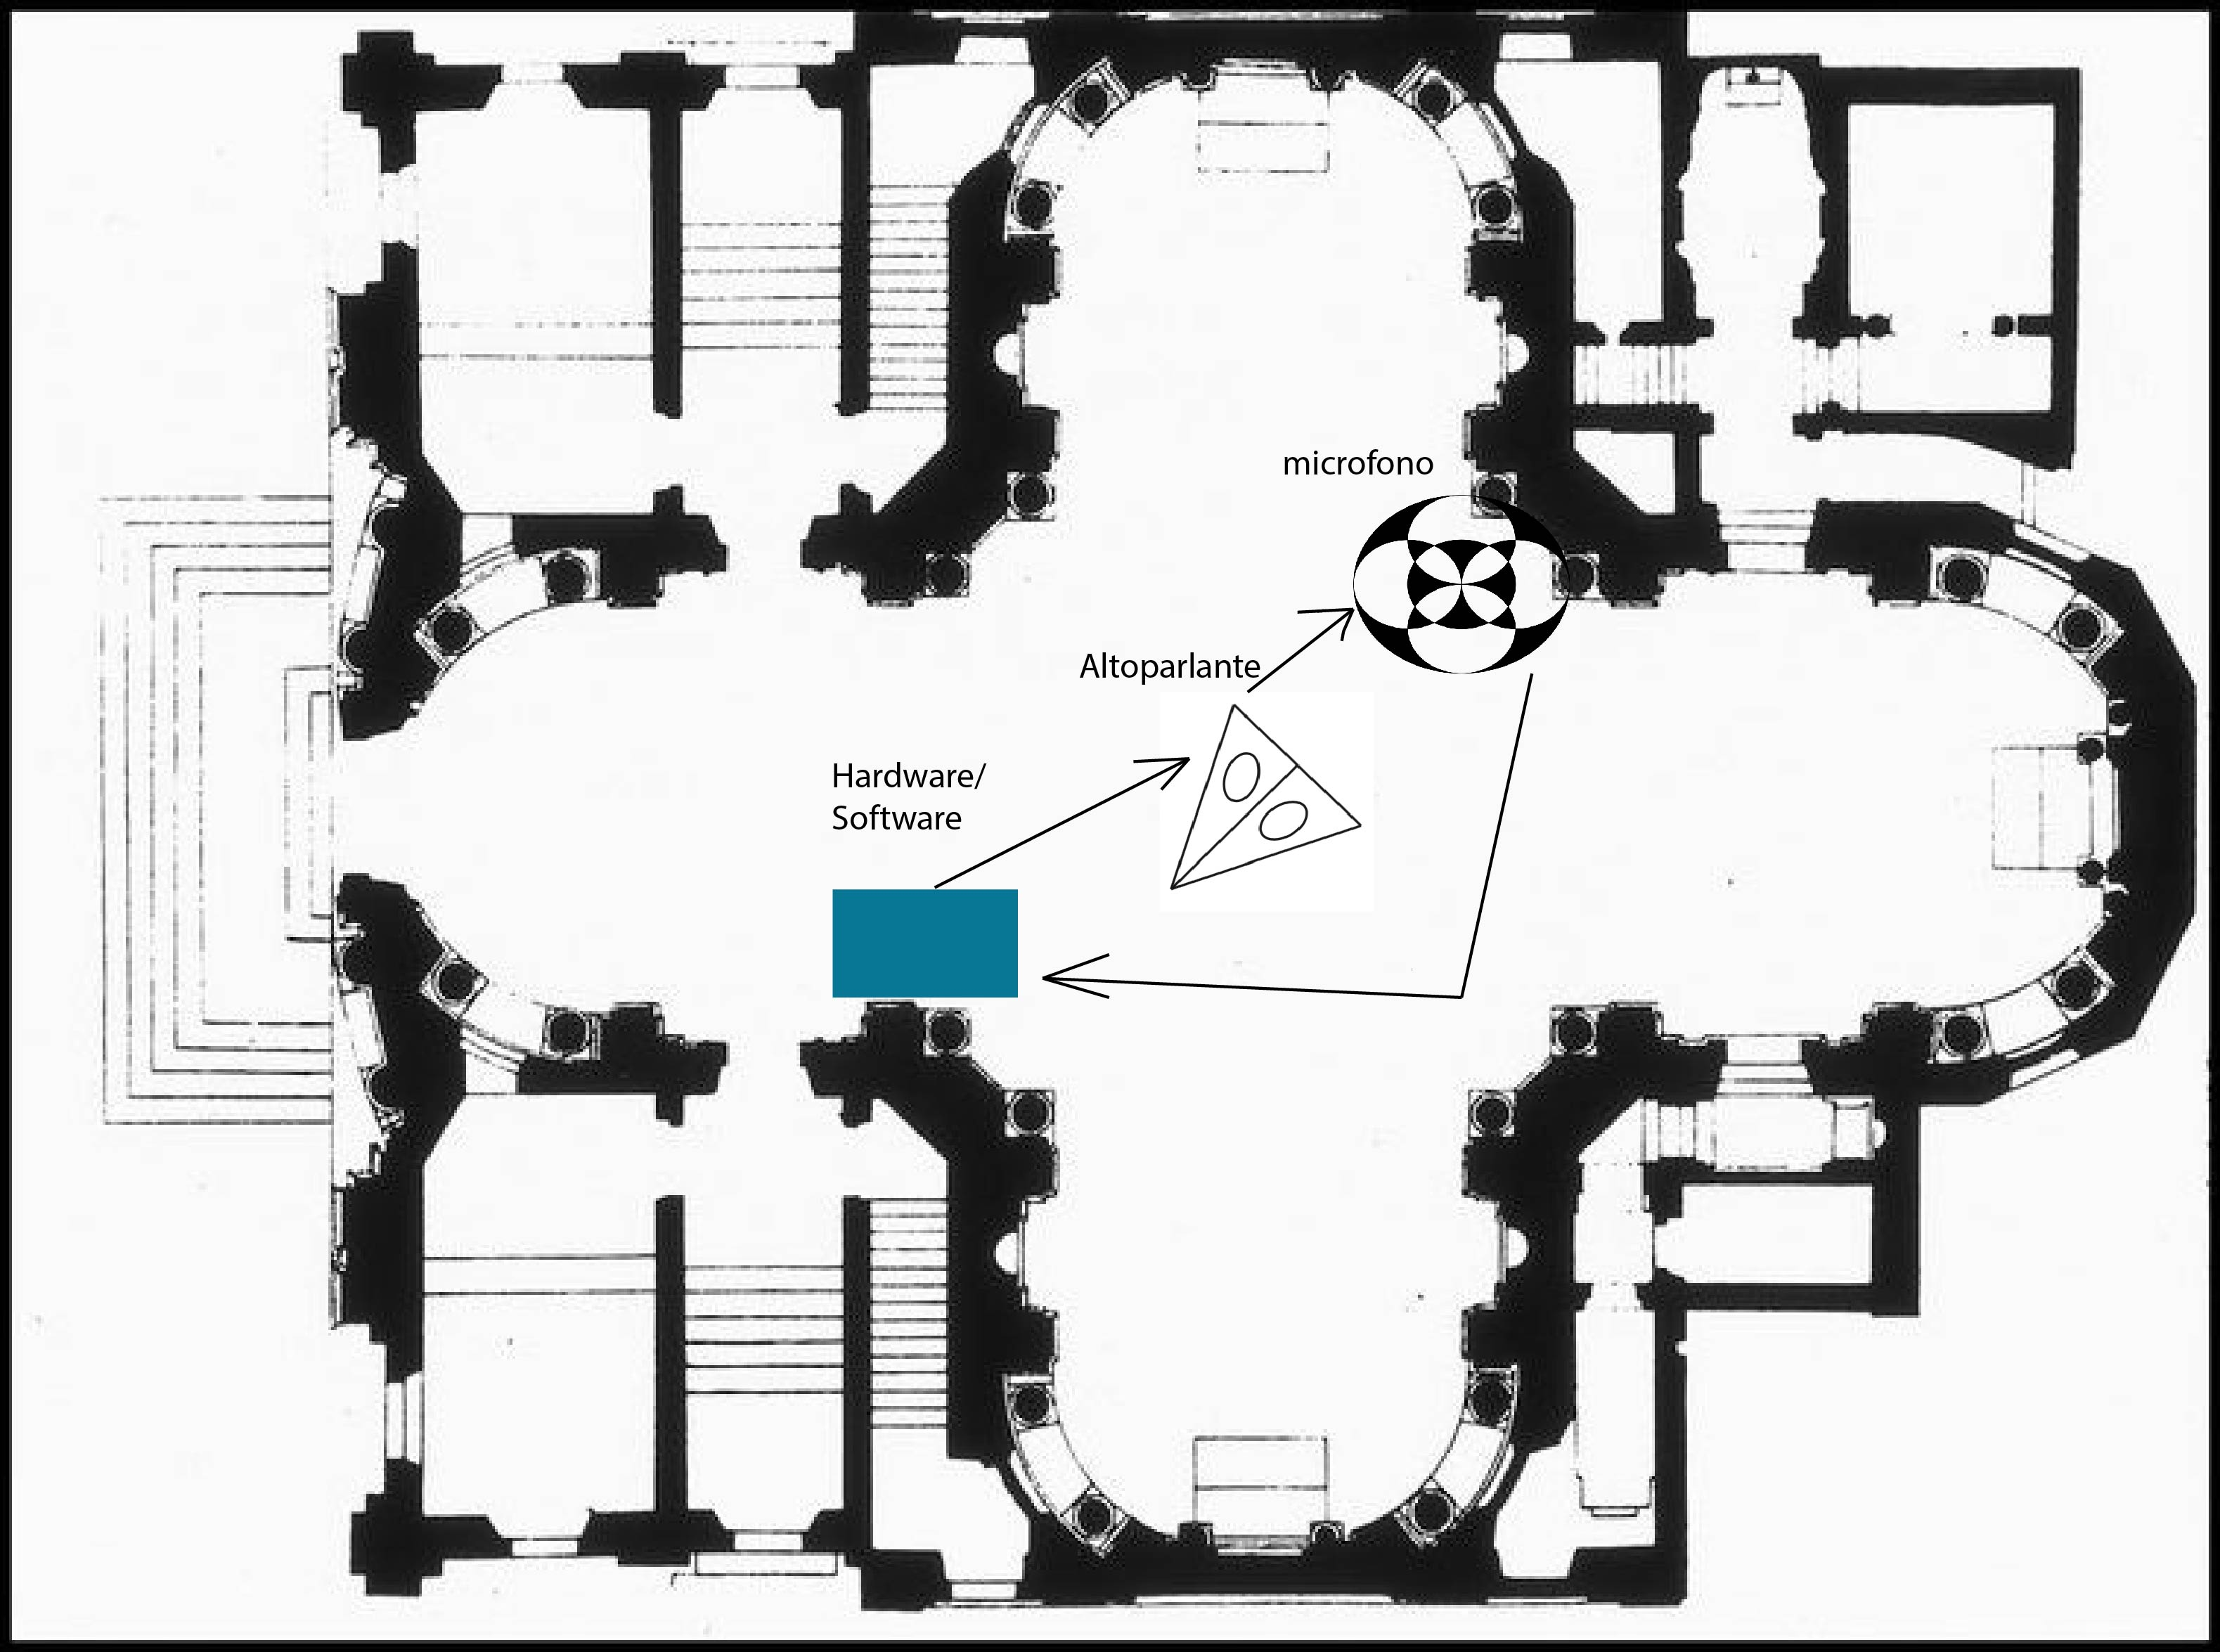
\includegraphics[width=.99\columnwidth]{file0031.jpg}}
\caption[Pianta S. Luca]{Catena di misurazione della risposta all'impulso}
\label{fig:tetratetra}
\end{figure}

\section{Risposta all'impulso}

Nel postulare le formule del nostro sistema lineare tempo invariante [LTI], Sabine ci rammenta
che questo sistema fisico  non deve  modificarsi nel momento di attuazione dell'analisi acustica.
L'LTI può essere rappresentato tramite una risposta all'impulso, ovvero misurare il suo
comportamento acustico.  Una sorgente, (nel nostro caso omnidirezionale) emette un
segnale $x(t)$  cui sarà sottoposto a modifiche del sistema:

dove

\begin{description}
	\item[$x(t)$] = segnale sorgente 
	\item[$F(x(t))$] = funzione di trasferimento
	\item[$n(t)$] = rumore ambiente
\end{description}

il segnale sorgente sarà comunque alterato dal trasduttore e dal rumore di fondo della stanza $n(t)$.

\begin{quote}

La risposta all'impulso $h(\tau)$ è la risposta del sistema nell'ipotesi che la
sorgente sonora generi un segnale $x(\tau)$ particolare, ossia un solo impulso unitario,
preceduto e seguito da una infinità di zeri. Esso è chiamato funzione delta di \emph{Dirac}:\footnote{3 Ivi. p. 5} 

\end{quote}

\begin{equation}
\delta(t) = 0~\textbf{per}~t~\neq 0~~~~~\int_{-\infty}^{+\infty}~\delta(t)dt=1
\end{equation}


Possiamo parlare della nostra risposta in Frequenza $H(f)$ (funzione di trasferimento),
come la  trasformata di \emph{Fourier} di $h(t)$: il prodotto tra gli spettri di $x$ e $y$ in funzione della frequenza

\begin{equation}
Y(f)= X(f)*H(f) 
\end{equation}

La funzione $F$ è prodotto di convoluzione tra il segnale di input e la risposta all'impulso del sistema

\begin{equation}
h(t):y(t)= n(t) + x(t) x h(t)
\end{equation}


\section{Scelta di distribuzione della sorgente e del microfono}

La peculiarità del progetto è quella di usare  quattro diffusori tetraedrici nella sala
da concerto per ri-descrivere lo spazio sonoro.

Il complesso sonoro tridimensionale è registrato tramite il microfono \emph{a-format}
messo nei quattro angoli del quadrato con il diffusore omnidirezionale al centro del quadrato. 

\begin{figure}
\centering
{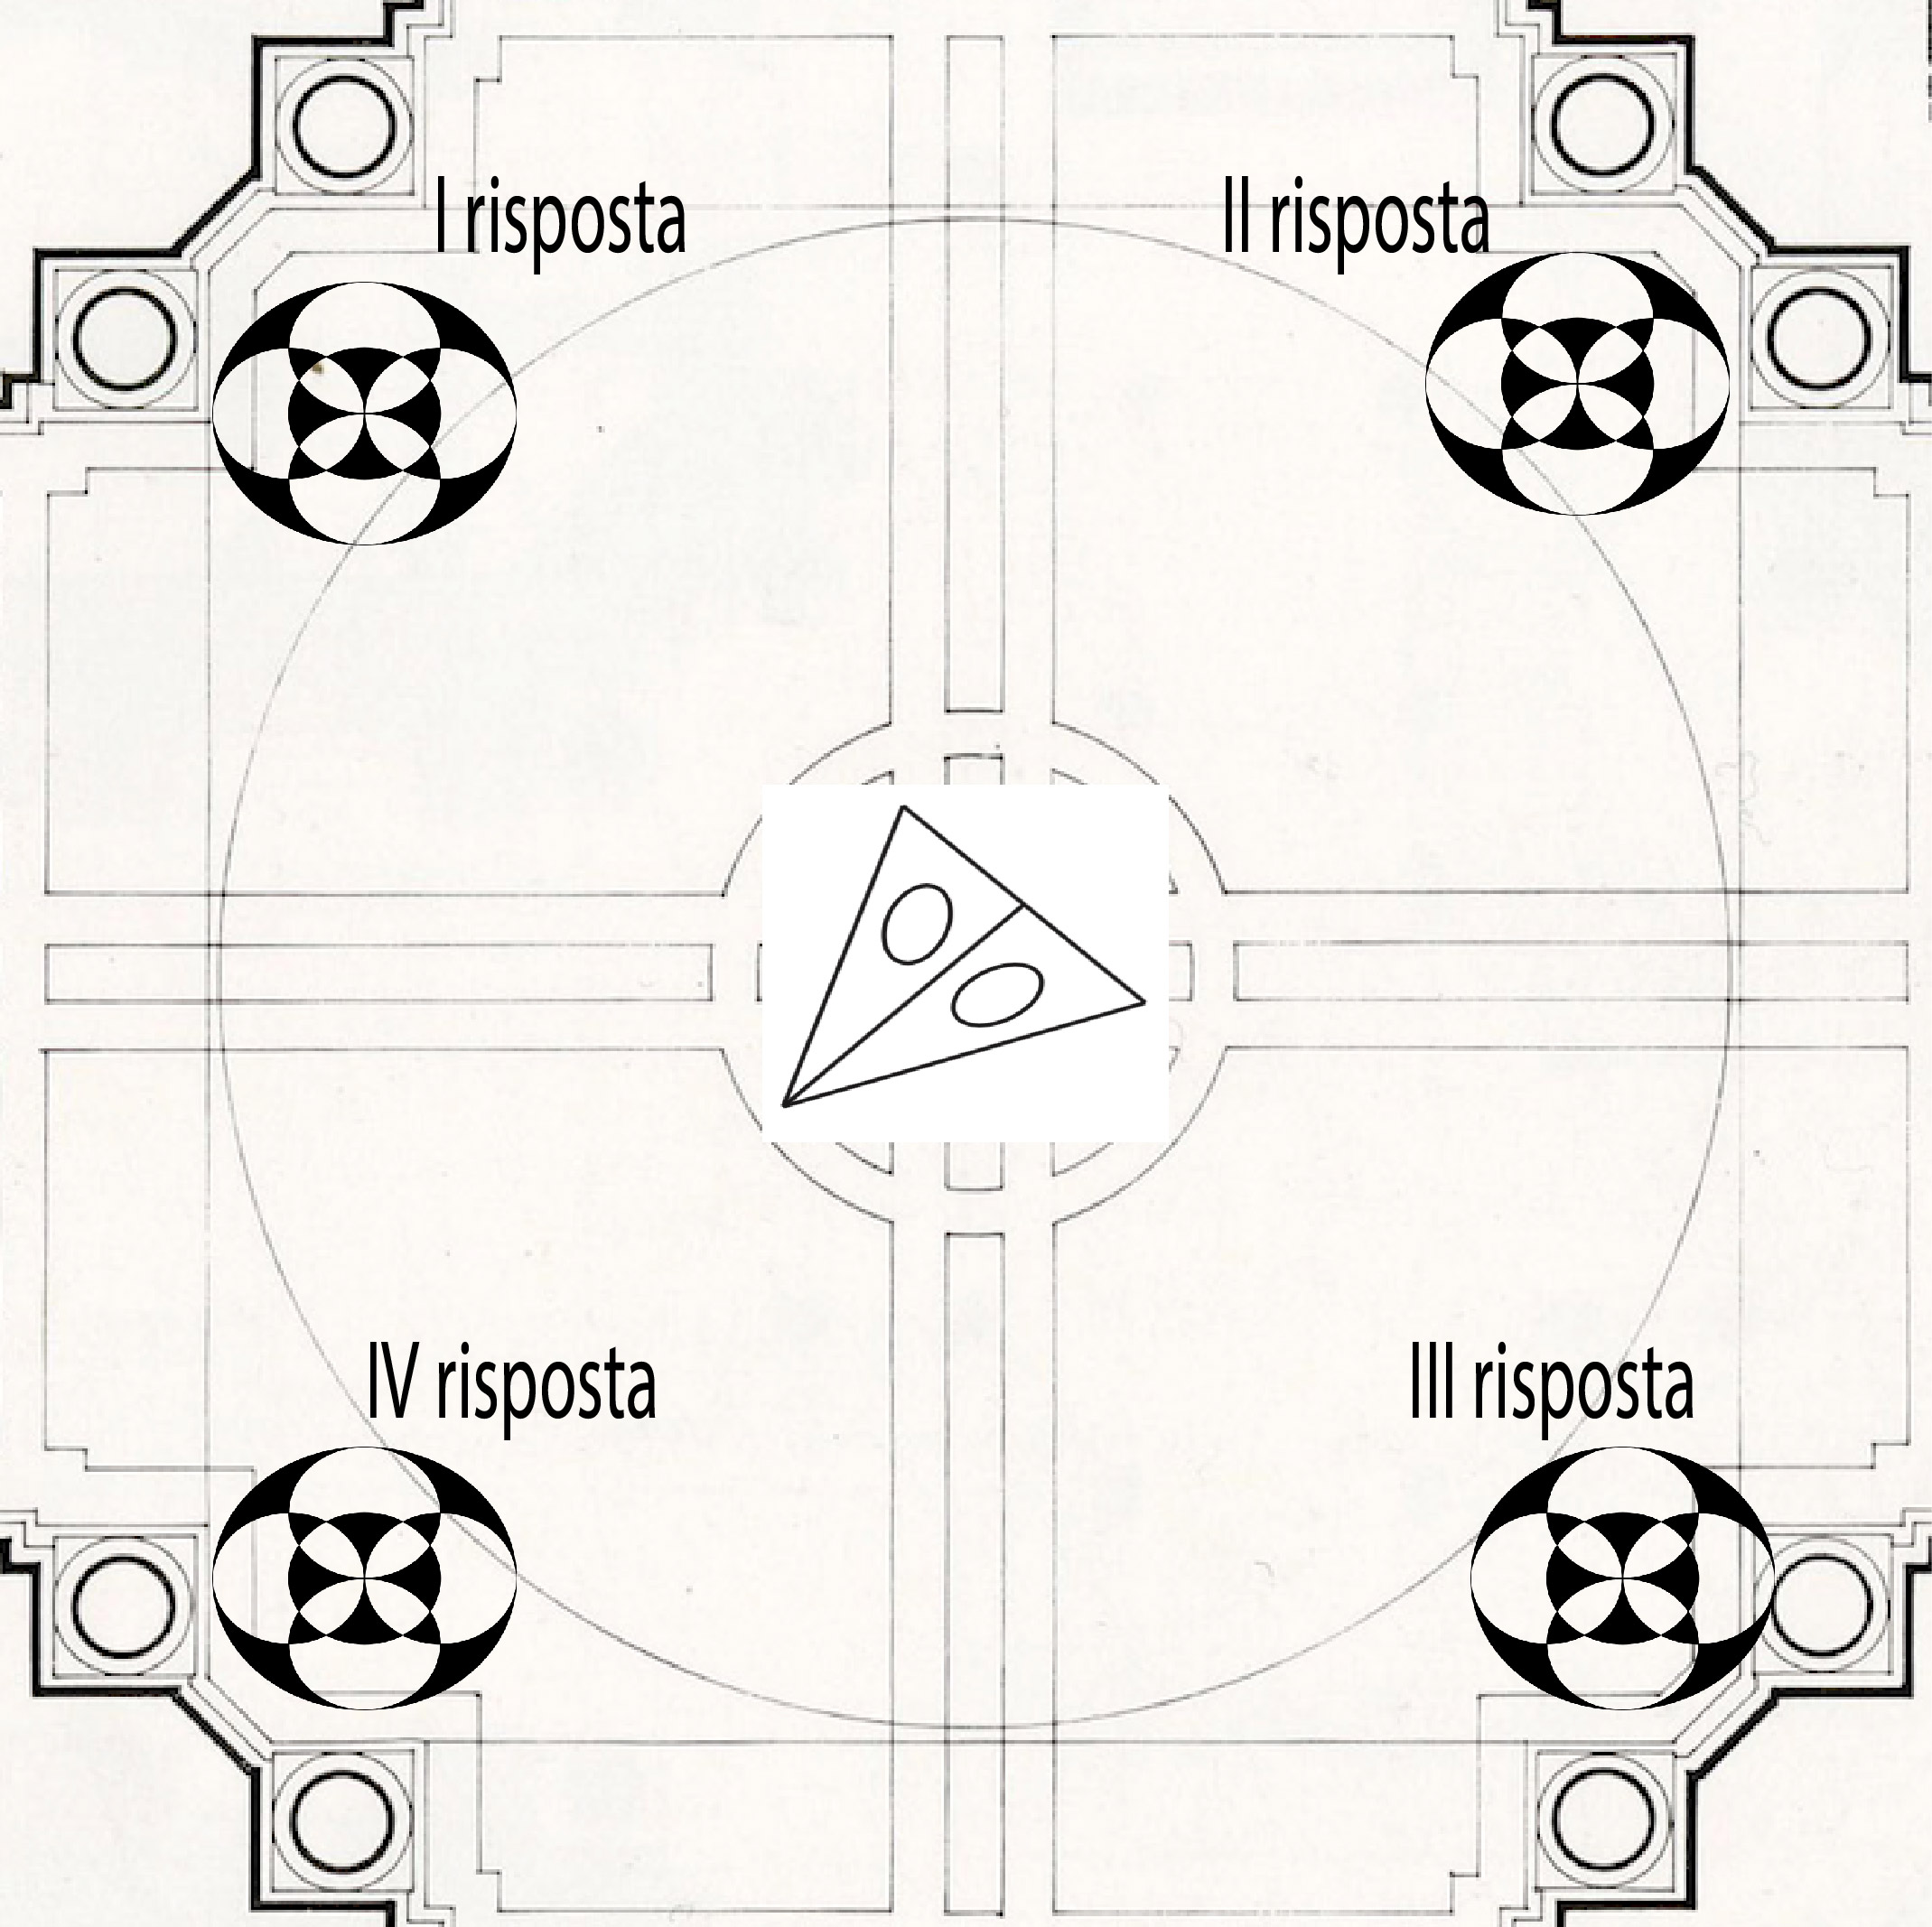
\includegraphics[width=.99\columnwidth]{file009.jpg}}
\caption[Pianta S. Luca]{Catena di misurazione della risposta all'impulso}
\label{fig:tetratetra}
\end{figure}

Le distanze sono state misurare ed equilibrate per dislocare i sistemi tetraedrici
facilmente nello spazio della sala.

\section{Strumentazione tecnica di misura}

La misurazione dell'ambiente ha fatto affidamento su questa strumentazione:

\begin{itemize}
	\item Mac Book pro portatile
	\item Finale di potenza t amp 700
	\item microfono A-format soundfield
	\item microfoni omni-direzionali dpa 4006
	\item microfoni omni-direzionali audio line OM1
	\item S.T.ONE
\end{itemize}

\section{Prova}

In un indagine di primo livello dall'acustica di San Luca è stato importante suonare
parte del brano con l'interprete all'interno della chiesa. Partendo da un concetto
di auralizzazione per poi via via affrancarsi dalla metodologia scientifica e ricavare
la propria risposta nell accoppiamento tra stanza virtuale e stanza reale, è stato
importante ricavare empiricamente le regioni che meglio soddisfavano le eseigenze
compositive. L'interprete ha eseguito parte del brano in diversi punti della navata,
portando all'attenzione le riflessioni e risonanze preponderanti. 
Le prove che hanno dato maggior riscontro acustico in funzione musicale riguardano
il centro della chiesa e la collanna di sinistra vicina al cenacolo.

la scelta di posizionamento del sistema tetraedrico interno alla chiesa per la
risposta all'impulso si è basata anche per il posizionamento possibile del sassofonista
in concerto.
Un possibile quadrante che inglobi il pubblico in concerto, corrispondente al
quadrante interno alla croce, dove sono ubicati i banchi da chiesa.
Come nel posizionamento dello STone per la risposta all'impulso, sono state
effettuate molteplici prove per sistemare per il quadrante ottimale. Di seguito
le configurazioni accettate per l'esecuzione:

\begin{figure}[h]
\centering
\subfloat[Asia personas duo]
{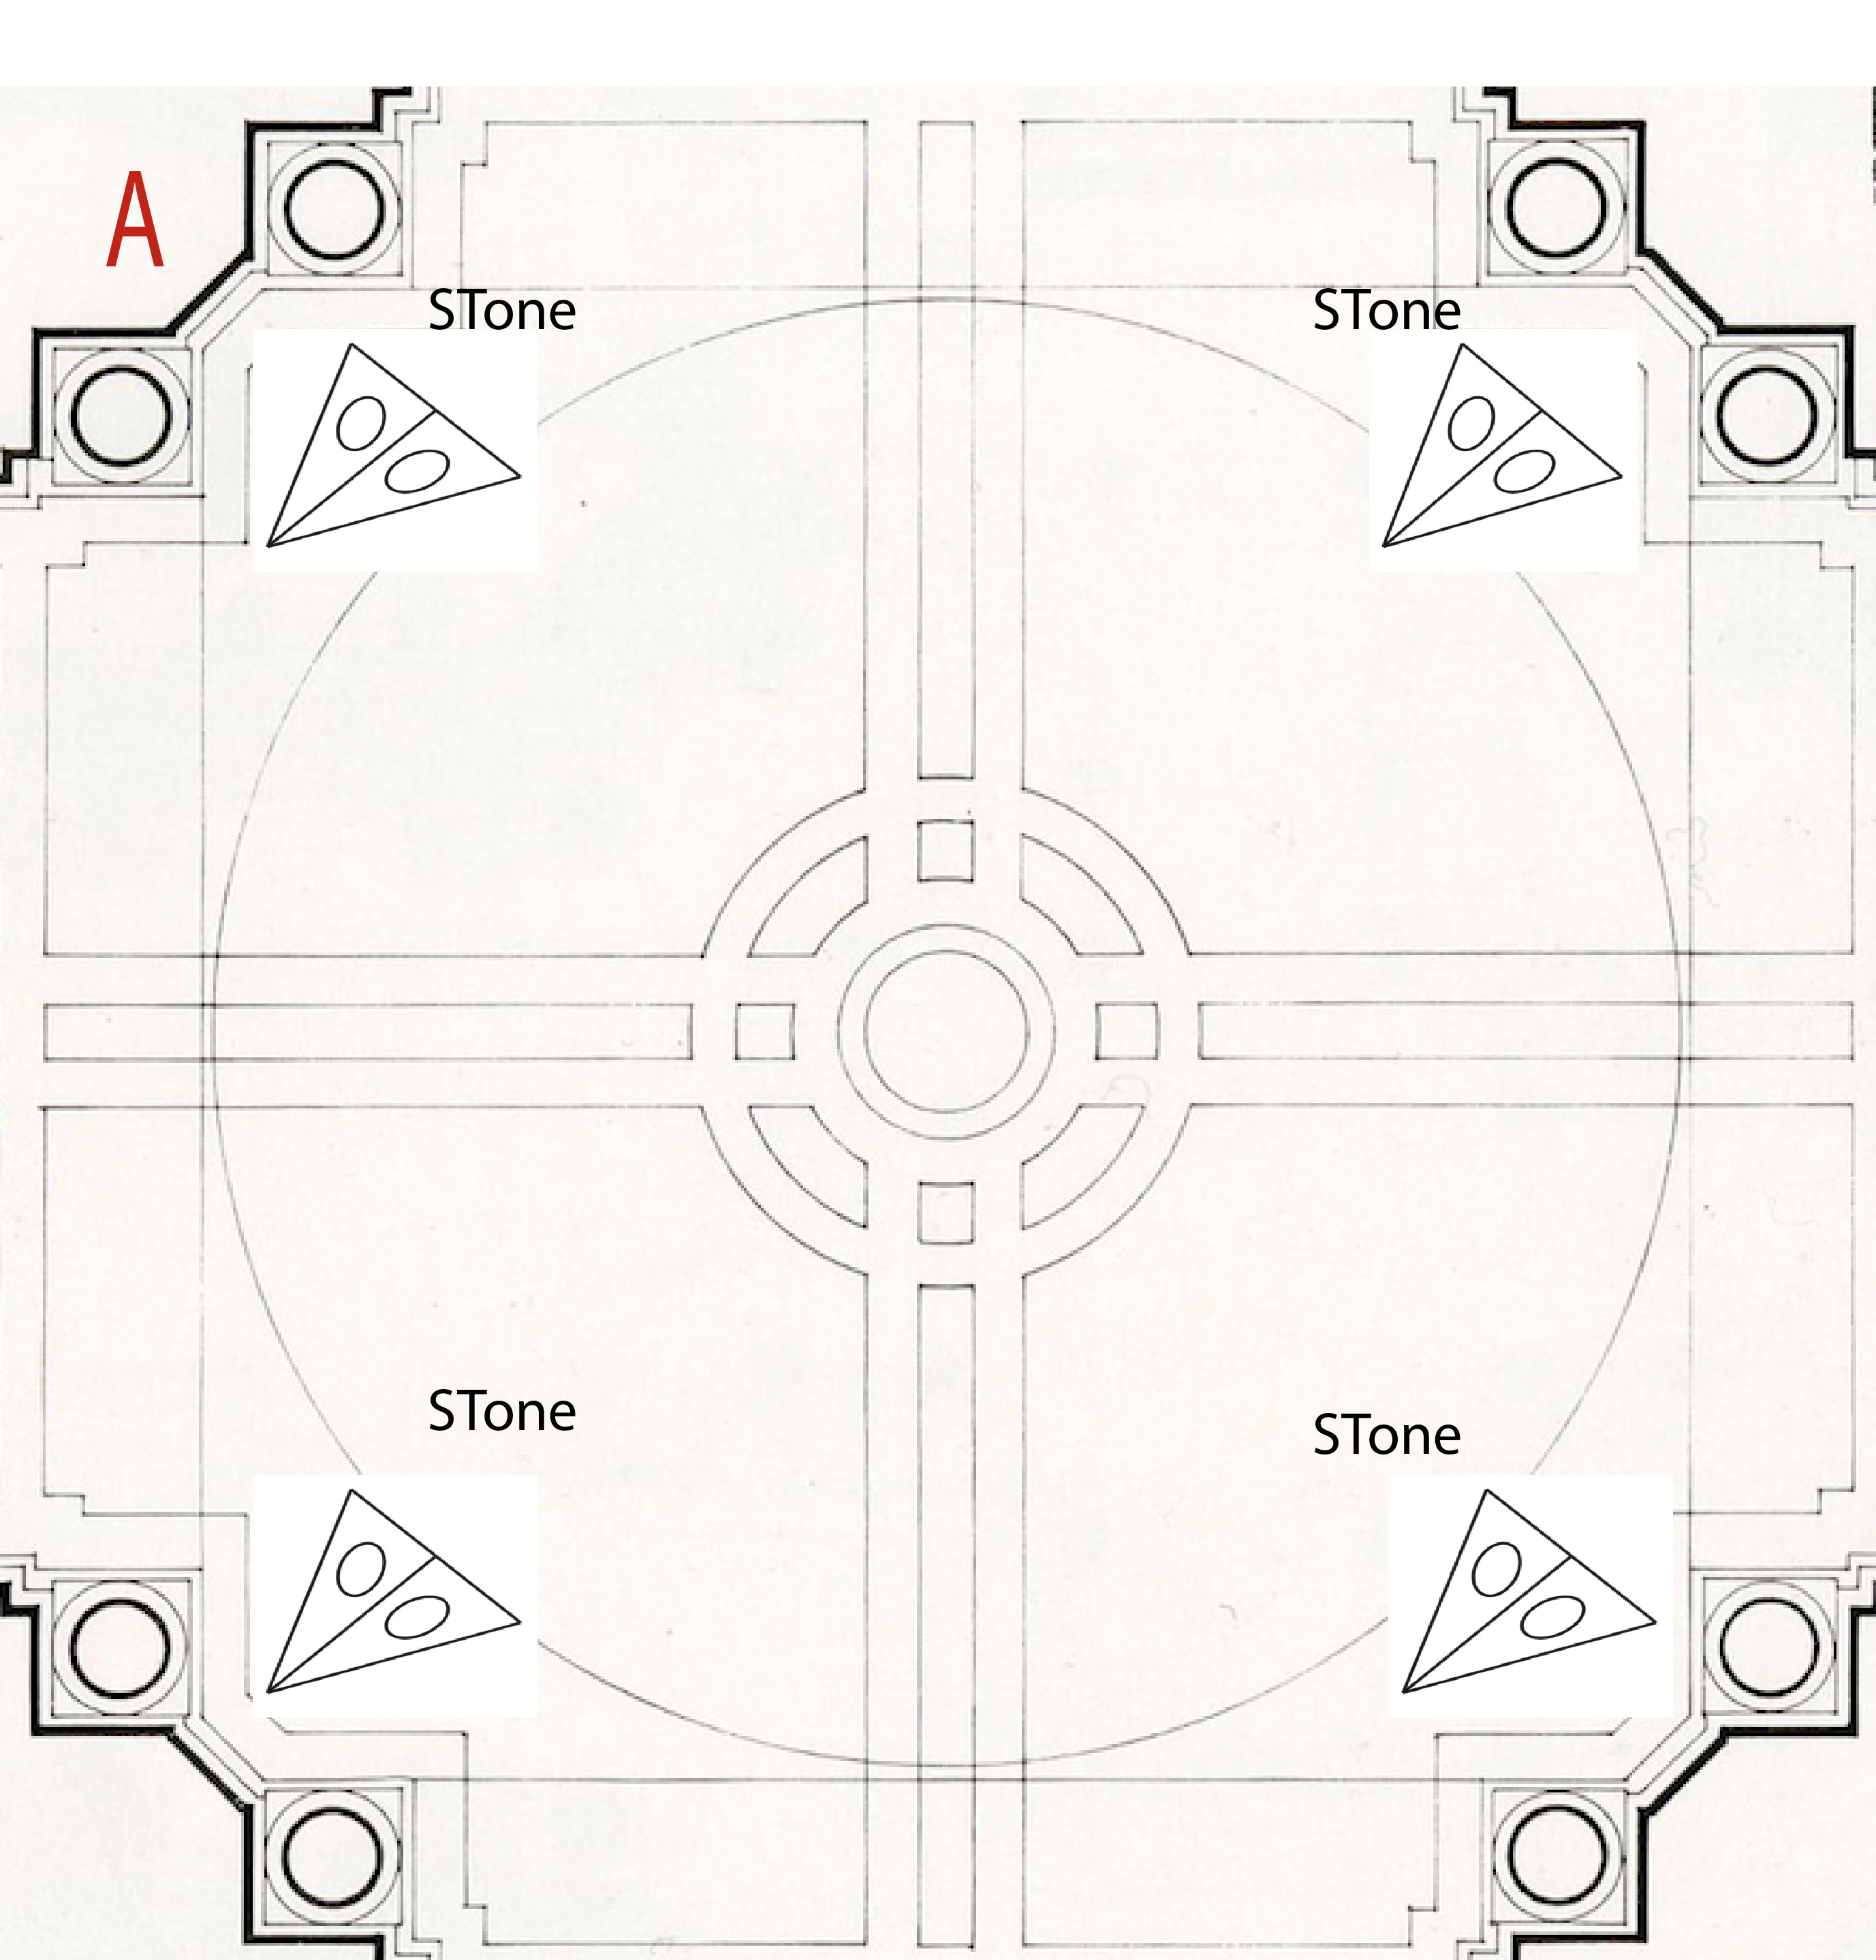
\includegraphics[width=.45\columnwidth]{file004.jpg}} \quad
\subfloat[Pan ma signo]
{\label{fig:example-b}%
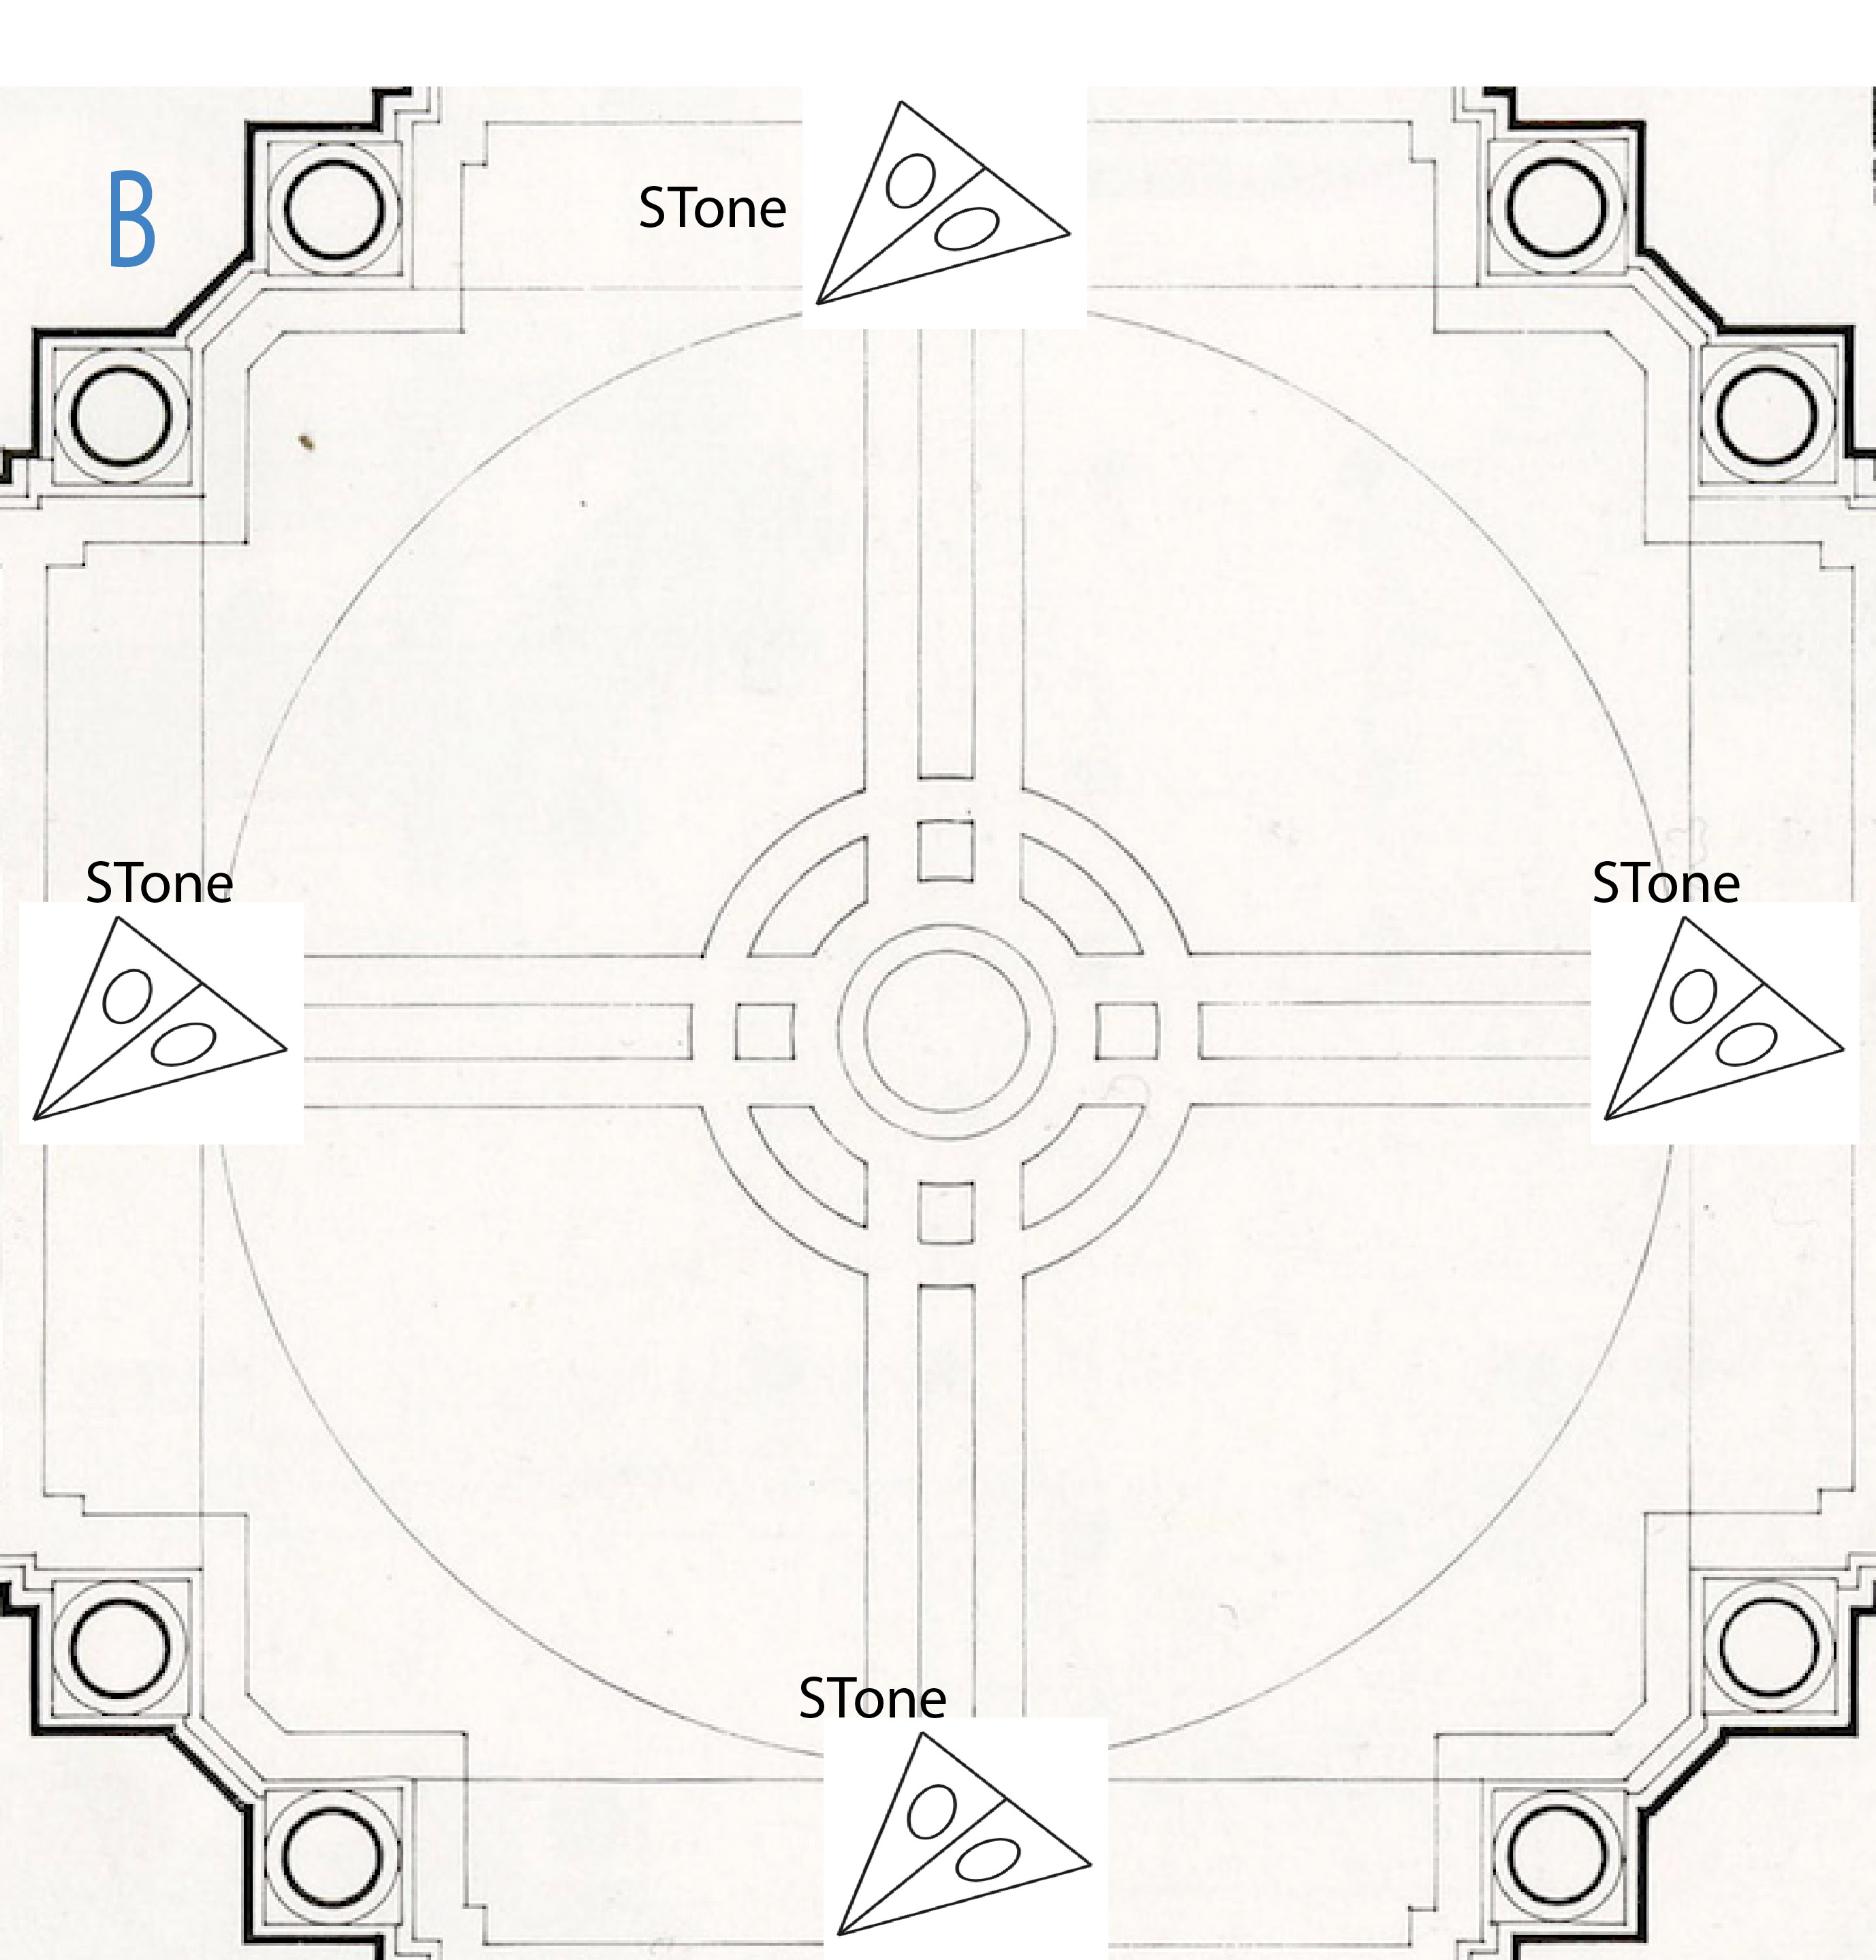
\includegraphics[width=.45\columnwidth]{file005.jpg}}
\end{figure}

La prima esecuzione prevista per il brano è stata alla Filarmonica Romana il
22/11/2016 e la conformazione della sala è un rettangolo: Questo ha escluso
la configurazione B di tipo "diamond" in quanto avremmo avuto l'interprete in
prospettiva dell'altoparlante e il ridimensionamento del quadrante formato dagli
Stone inscritto,rispetto alla configurazione A che non presentava questo tipo di inconveniente.

\section{Impulse Response Retrieval} 

La tecnica di misurazione adottata fa affidamento al descrittore acustico di tipo ESS.
Essendo la chiesa vicino ad un via molto trafficata e con possibilità di rumore di
fondo molto alta, si era pensato di determinare le caratteristiche dell'ambiente
tramite sistema MlS, maximum length sequences. 
Ricordiamo che questa tecnica mette in correlazione segnale di ingresso $ x(n) $
e segnale di uscita $ y(n) $ di un sistema lineare. 
In pratica si applica questa sequenza pseudocasuale (simile ad un rumore bianco)
all'ingresso del sistema e moltiplicando poi questo segnale in uscita con la
sequenza iniziale di ingresso. Il risultato è la funzione delta di Dirac:

Questa misurazione permette un ottimo bilanciamento suono/rumore di fondo,
anche in condizioni molto precarie.
Ma il metodo  di sweep (lineare o esponenziale che sia) permette un risulatato
migliore al fronte di distorsione armoniche del sistema (altoparlante).

Metodo ESS (exponential sine sweep)

Il nostro descrittore acustica è uno segnale sweep esponenziale, che si sviluppa nel tempo.
Partendo da una sequenza dal di sopra del dc. 
La frequenza si raddoppia ripetutamente a tempi di intervallo indentico.

Tempo ed energia sono spese per partire dalla bassa frequenza fino alle alte:

si è partiti da una frequenza di 30 HZ fino a 22000 HZ:
per partire a frequenze cosi basse è stato integrato un sub woofer.

A differenza di un chirp lineare si possono raccogliere maggiori informazioni selle frequenze percepite. 

EQUAZIONE \\
------file006-----

w1 frequenza di partenza normalizzata in radianti (frequenza angolare iniziale)

w2 è la frequenza di arrivo in radianti (frequenza angolare finale)

n è l'indice dei sample

n è il numero dei samples

Anche questo sistema porta con se, oltre all'effetto di riverbero della stanza anche
le componenti di rumore e gli effetti di distorsione non lineare di cui parlavamo in
precedenza (dirsione della fondamentale della componente elettronica)

Anche per quanto riguarda l'ampiezza il segnale è costante tutto il tempo. L'analisi
mostra un decay della magnitudine di 6 db per ottava. Questo decay della magnitudine
viene compensato quando la risposta all'impulso è calcolata tramite deconvoluzione,
in quanto la compensazione è fatta nel domnicio digitale e non altera il rapporto
segnale rumore favorendo la gamma di bassa frequenza del segnale di prova.

Vista la registrazione di molteplici risposte bisogna arrivare alla maggior efficenza
del sistema.
 Lo spettro registrato non risulta perfetto in quanto caratterizzato da frequenze di
 ripple agli estremi, che in taluni casi superano i + 5 db. I confini del chirp ( di start e di stop)
 presentano queste frequenze indesiderate, causa anche la parziale cancellazione di fase e somma sopra il segnale. 


chirp expo:2.5 further ripple reduction: fade-in window  e deconvoluzione

segnale di putput y(t)convoluto con il filtro inverso

risposte markidis


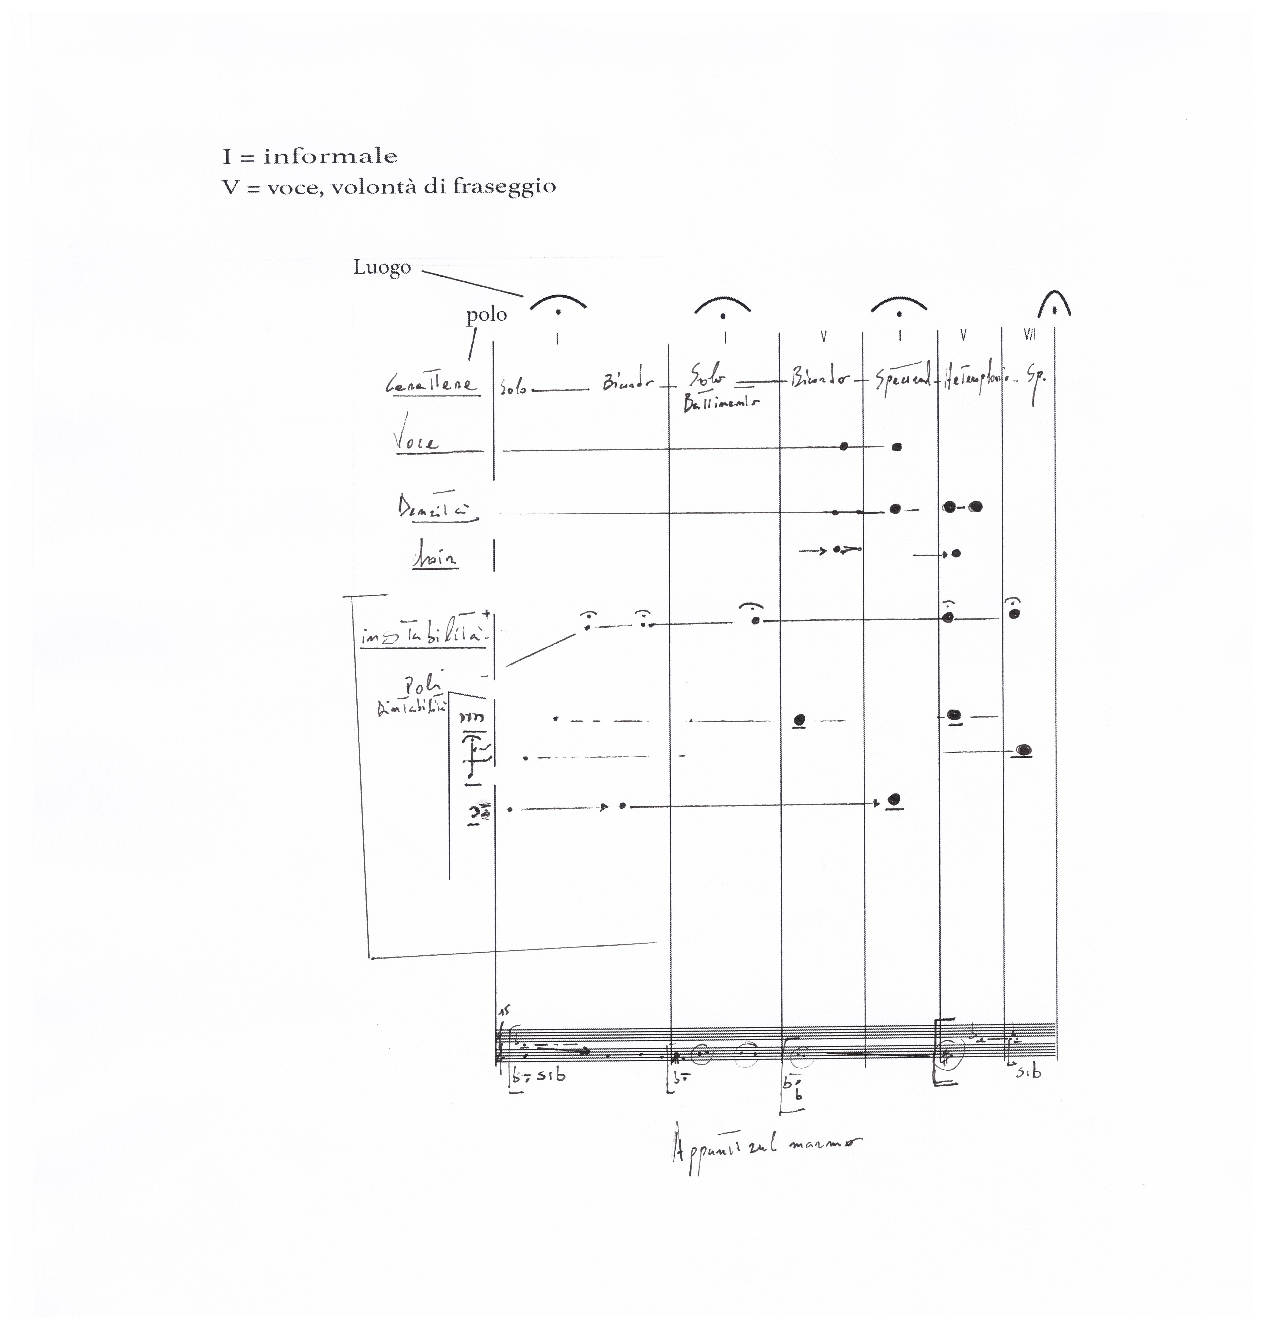
\includepdf[scale=1.3, offset=10 0]{macrostruttura.pdf}